\documentclass[a4paper,12pt]{article}

\usepackage{graphicx}
\usepackage{amsmath}
\usepackage{setspace}
\usepackage{url}
\usepackage{caption}
\usepackage{subcaption}
\usepackage{placeins}

%Title page
\title{
    \vspace{15pt}
    \textbf{A Comparative Study of NumPy and TensorFlow Implementations of a Multilayer Perceptron on MNIST} \\
    \vspace{15pt}
    \large Analysing optimisation behaviour, numerical stability, and computational efficiency
}
\author{William T. Davies}
\date{\today}

%Main document
\begin{document}

\maketitle

\begin{abstract}
The optimisation behaviour of neural networks is shaped not only by model architecture but also by the computational framework used to implement them. This work presents a controlled comparison between two implementations of an identical MLP trained on MNIST: a fully manual NumPy model with explicitly coded forward and backward passes, and a TensorFlow/Keras model employing automatic differentiation and optimised tensor kernels. The aim is to isolate the effect of implementation strategy on convergence stability, numerical robustness, and computational efficiency. Using a structured grid of batch sizes and learning rates, and averaging results across repeated trials, we observe that TensorFlow delivers smoother optimisation trajectories, higher and more consistent test accuracy, and markedly faster training—particularly at large batch sizes where kernel-level parallelism is most effective. The NumPy implementation displays higher variance, noisier learning curves, and training times largely insensitive to batch size, while still offering valuable pedagogical insight. These findings demonstrate that implementation-level choices materially influence learning dynamics, even for simple models, and highlight the practical importance of using optimised deep-learning frameworks in applied settings.
\end{abstract}

\thispagestyle{empty} 
\newpage

\pagenumbering{roman}
\setcounter{page}{2}

\begin{spacing}{2}
\tableofcontents
\end{spacing}

\newpage
\pagenumbering{arabic}





\section{Introduction}
\subsection{Background and Motivation}
Foundational machine learning models continue to play an important role in both research and education, despite the rapid development of increasingly complex architectures. Simple multilayer perceptrons (MLPs) remain a valuable benchmarking tool: they are expressive enough to capture meaningful structure in data, yet sufficiently compact to allow detailed inspection of their optimisation dynamics. Their transparency makes them ideal for controlled experiments in which the mechanisms of forward and backward propagation, gradient flow, and generalisation behaviour can be studied with minimal architectural confounding factors.\\

The MNIST handwritten digit dataset has, for decades, served as a canonical benchmark for such investigations. Its modest dimensionality, balanced class distribution, and well-understood difficulty profile make it an ideal platform on which to compare optimisation strategies, implementation choices, and computational trade-offs. Although MNIST is no longer considered a challenging problem in modern machine learning, its simplicity allows the focus to shift away from representational capacity and toward the behaviour of training procedures themselves.\\

Implementing an MLP from first principles provides educational value that extends beyond raw performance. A hand-crafted NumPy model reveals, explicitly, each mathematical operation required for prediction and gradient computation. This transparency is pedagogically useful: it exposes the consequences of different design decisions, numerical instabilities, and the computational bottlenecks inherent in pure Python implementations. In contrast, deep learning frameworks such as TensorFlow hide many of these details behind automatic differentiation engines and heavily optimised kernels. Although these frameworks are indispensable for large-scale applied work, it is often unclear how much of their performance advantage stems from algorithmic differences versus purely computational optimisations.\\

This study is motivated by the opportunity to contrast these two philosophies directly: a manual NumPy-based implementation, in which all operations and gradients are explicitly defined, and a TensorFlow implementation, which leverages automatic differentiation, vectorised operations, and hardware-optimised execution. By fixing the model architecture and dataset, the analysis isolates how the implementation strategy itself shapes optimisation behaviour, runtime performance, and sensitivity to hyperparameter choices.\\

\subsection{Objectives of the Study}

The primary objective of this work is to rigorously evaluate how two implementations of the same multilayer perceptron behave under identical experimental conditions. To this end, the study aims to compare the NumPy and TensorFlow models along several key dimensions:
\begin{itemize}
\item Training speed: quantifying the computational efficiency of each implementation, with particular attention to how batch size influences runtime in pure Python versus optimised kernels.
\item Test accuracy: assessing the generalisation performance achieved across a grid of learning rates and batch sizes.
\item Sensitivity to hyperparameters: analysing how each model responds to changes in learning rate and batch size, and identifying systematic trends or instabilities.
\item Stability and convergence behaviour: comparing the smoothness and monotonicity of loss curves, the consistency of optimisation trajectories across trials, and the susceptibility to noisy or erratic gradients.
\end{itemize}

Collectively, these objectives provide insight into the extent to which performance differences arise from the underlying mathematics of gradient descent versus the engineering optimisations present in modern deep learning frameworks. The comparison illustrates the practical impact of implementation choices on both accuracy and computational efficiency, thereby highlighting the trade-offs between educational clarity and applied performance.

\section{Dataset}
\subsection{Overview of MNIST}

The MNIST handwritten digit dataset is a well-established benchmark in machine learning and pattern recognition. It contains 70,000 grayscale images of handwritten digits, each of resolution 28 × 28 pixels, yielding an input dimensionality of 784 features when flattened into a vector. The dataset covers 10 classes corresponding to the digits 0–9, with a balanced distribution across categories.\\

For experimentation, MNIST is conventionally partitioned into a training set of 60,000 images and a test set of 10,000 images, a split that is preserved in this study. Each example consists of a single-channel intensity map with integer pixel values in the range 0–255.\\

To maintain consistency across implementations, the following preprocessing steps were applied:

\begin{itemize}
\item	Normalisation: all pixel values were scaled by a factor of 1/255, mapping inputs to the range [0,1].
\item Flattening: each image was reshaped into a 784-dimensional vector, as required for fully connected MLP architectures.
\item Label formatting: labels were stored as integer class indices, with no one-hot encoding performed explicitly in the NumPy implementation (the loss function operates directly on index labels).
\end{itemize}

No additional preprocessing—such as whitening, standardisation, augmentation, or dimensionality reduction—was applied. This ensures that differences in training dynamics arise solely from the model implementations rather than from data transformations.\\

\subsection{Justification for using MNIST}

MNIST remains one of the most widely used standardised benchmark datasets for evaluating the behaviour of machine learning algorithms under controlled conditions. Its key advantage in this context is that it isolates model behaviour rather than model capacity. Because MNIST is relatively simple by modern standards, the representational limitations of a small MLP do not dominate the results; instead, the focus naturally shifts to how implementation choices affect optimisation, runtime, and stability.\\

The dataset’s computational lightness is also a significant practical benefit. Its moderate size allows for: extensive hyperparameter sweeps across multiple batch sizes and learning rates, repeated trials to average out stochasticity in shuffling and weight initialisation, and full training of both NumPy and TensorFlow models without requiring GPU acceleration or long execution times.\\

By providing a clean, homogeneous evaluation environment, MNIST enables a fair and interpretable comparison between a manually coded NumPy model and an optimised TensorFlow model. The simplicity of the dataset ensures that observed differences in performance stem predominantly from implementation-level considerations—such as vectorisation, automatic differentiation, and kernel-level optimisations—rather than from the representational challenges posed by the task itself.\\


\section{Model Architecture}
\subsection{Multi-Layer Perceptron Structure}

Both the NumPy and TensorFlow implementations employ an identical multilayer perceptron (MLP) architecture to ensure that all observed differences in performance arise solely from implementation details rather than from model design.
The network accepts a 784-dimensional input vector, corresponding to the flattened 28 × 28 MNIST image. This input layer feeds into a single hidden layer consisting of 64 neurons, a common size that provides sufficient representational capacity for MNIST while remaining computationally manageable for a from-scratch implementation.\\

The hidden layer uses the rectified linear unit (ReLU) activation function. ReLU is chosen for its simplicity, favourable gradient properties, and widespread use in modern neural networks. It avoids the vanishing-gradient issues associated with sigmoidal activations, which would be particularly damaging in a manually implemented model lacking the stabilising heuristics found in large frameworks.\\

The output layer consists of 10 neurons, one for each digit class. A softmax transformation is applied to produce a normalised probability distribution over classes. This allows training to proceed using cross-entropy loss in both implementations, ensuring full comparability between optimisation behaviour and prediction performance.
Thus, the architecture can be summarised as:

\begin{itemize}
\item Input: 784
\item Hidden Layer: 64 units, ReLU activation
\item Output Layer: 10 units, softmax activation
\end{itemize}

\subsection{Design Rationale}

The architectural choices in this study are intentionally minimalistic. The goal is not to pursue state-of-the-art accuracy on MNIST, but rather to create a controlled setting in which the computational and optimisation differences between two implementation paradigms can be meaningfully compared.
A simple, shallow MLP was selected for three principal reasons:
First, simplicity promotes a fair comparison. By restricting the model architecture to its most basic form, the study removes any confounding factors arising from complex components such as convolutional filters or deep hierarchical structures. What remains is a pure comparison of how the two frameworks execute the same mathematical operations.
Second, the model is deliberately chosen to be easy to express identically in NumPy and TensorFlow. A single hidden layer with ReLU and softmax avoids subtle discrepancies—such as different initialisation defaults, normalisation layers, or fused kernel implementations—that could influence results in ways unrelated to the underlying optimisation process.
Third, an MLP remains fully appropriate for MNIST. Although convolutional neural networks outperform MLPs on this task, the MLP achieves respectable accuracy, captures the core structure of the data, and trains quickly. This aligns with the study’s emphasis on investigating training dynamics, convergence behaviour, and computational cost rather than maximising predictive accuracy.

\section{Implementation Details}
\subsection{NumPy Implementation}

The NumPy model is implemented entirely from first principles, with all computational steps defined explicitly. Forward propagation is carried out using matrix multiplications followed by nonlinear activations. Given an input batch X, the first affine transformation is computed as

\begin{equation}
z_1=XW_1+b_1
\end{equation}

and the hidden activations are obtained through the ReLU function,

\begin{equation}
a_1 = \operatorname{ReLU}(z_1) = \max(0, z_1)
\end{equation}

The output logits are then produced via the second affine map,

\begin{equation}
z_2=a_1 W_2+b_2
\end{equation}

After which a softmax transformation converts logits into class probabilities,

\begin{equation}
\hat{y}_i= \frac{\exp{z_{2,i}} } {\sum_j\exp{z_{2,j}}}
\end{equation}

Each of these operations is implemented with standard NumPy array functions, ensuring complete transparency of the underlying calculations.
The compact final equation for the forward pass is as follows:

\begin{equation}
\hat{y} =\operatorname{softmax}(\operatorname{ReLU}(XW_1+b_1)W_2+b_2)
\end{equation}

Backward propagation is likewise implemented manually. The loss for a single sample, using cross-entropy with softmax, is

\begin{equation}
L = -\log(\hat{y}_{y})
\end{equation}

Where $\hat{y}_y$ is the predicted probability assigned to the true class $y$. Differentiating the softmax–cross-entropy composition yields a simple expression for the output-layer error term,

\begin{equation}
\delta_2=\hat{y}-y_{\operatorname{onehot}}
\end{equation}

Which forms the starting point of the manual backpropagation chain. The gradients of the loss with respect to the second-layer parameters follow directly:

\begin{equation}
\frac{\partial L}{\partial W_2} = a_1^{\top} \delta_2, 
\quad\text{and}\quad
\frac{\partial L}{\partial b_2} = \delta_2
\end{equation}

Propagating the error through the ReLU nonlinearity requires masking by the indicator of positive preactivations,

\begin{equation}
\delta_1=(\delta_2 W_2^\top)\odot1_{(z_1>0)}
\end{equation}

After which the first-layer gradients are obtained as

\begin{equation}
\frac{\partial L}{\partial W_1} = X^\top \delta_1,
\quad\text{and}\quad
\frac{\partial L}{\partial b_1} = \delta_1
\end{equation}

These derivations, implemented directly using NumPy broadcasting and matrix operations, make the gradient flow through the network fully explicit, exposing the Jacobian structure of the MLP and the precise manner in which errors propagate backward.\\

Weights are initialised using a He-uniform scheme with sampling range

\begin{equation} 
W \sim U(-\sqrt{\frac{6}{n_\mathrm{in}}}, \sqrt{\frac{6}{n_\mathrm{in}}}) 
\end{equation}

Ensuring appropriate variance scaling for ReLU activations. Biases are initialised to zero. Training proceeds through a Python-level loop: at the start of each epoch, the dataset is shuffled; each mini-batch is passed through forward propagation, gradients are manually computed using the expressions above, and parameters are updated using vanilla stochastic gradient descent,

\begin{equation}
W\leftarrow W- \alpha \frac{\partial L} {\partial W}, 
\quad\text{and}\quad
b\leftarrow b- \alpha \frac{\partial L} {\partial b} 
\end{equation}

After each epoch the full training set is evaluated to record loss and accuracy histories.
While this implementation is mathematically correct and pedagogically valuable, it exhibits inherent limitations. Pure Python loops restrict computational throughput and prevent efficient parallelisation, making runtime largely insensitive to batch size. The absence of GPU support confines execution to CPU-bound NumPy operations, dominated by interpreter overhead. Numerical stability must also be managed manually—for example, by shifting logits before exponentiation or clipping predicted probabilities—without the fused, stabilised kernels provided by industrial-grade frameworks.\\

\subsection{TensorFlow Implementation}

The TensorFlow version of the model is implemented using the Keras Sequential API, which provides a concise and modular interface for defining neural architectures. The structure mirrors the NumPy model exactly: a dense layer with 64 ReLU units followed by a 10-way dense softmax classifier. However, the implementation abstracts away the low-level mathematical details.\\

Optimisation is handled through TensorFlow’s high-performance runtime. The model is compiled with a categorical cross-entropy loss and a stochastic gradient descent optimiser configured with the same learning rates used in the NumPy experiments. TensorFlow automatically manages gradient computation through its autograd system, which constructs a dynamic computational graph and performs reverse-mode differentiation during the backward pass.\\

Although the experiments were conducted on CPU, TensorFlow preserves the abstraction between CPU and GPU execution. All operations are expressed as vectorised tensor kernels, and when run on GPU-enabled hardware, the same code would execute using highly parallel CUDA-backed implementations. Even in CPU-only settings, TensorFlow invokes optimised routines, improving computational efficiency relative to manually coded NumPy loops.\\

The framework also handles numerical stabilisation internally. Kernels for softmax, cross-entropy, and affine transformations are fused, reducing redundant computation and mitigating floating-point error accumulation. This leads to smoother and more stable optimisation trajectories, particularly at larger learning rates.\\

\subsection{Differences Between the Two Implementations}

The two models implement the same mathematical architecture, but their execution strategies differ fundamentally.
The NumPy model relies on manually coded gradients, expressed directly through algebraic operations. TensorFlow, by contrast, uses automatic differentiation, constructing and traversing a computation graph to compute gradients efficiently and reliably. This distinction is central to the comparison: while the NumPy code exposes gradient flow explicitly, TensorFlow isolates the user from these details and ensures correctness through its autodiff engine.\\

Execution modes also differ. The NumPy implementation uses pure Python eager execution, operating step-by-step through Python loops. TensorFlow, even in eager mode, performs most operations through compiled vectorised kernels that invoke BLAS or Eigen libraries. As a result, TensorFlow benefits from instruction-level parallelism, optimised memory layouts, and improved cache utilisation. NumPy’s operations are vectorised as well, but the presence of Python-level iteration in the training loop prevents the same degree of throughput.\\

Memory usage follows different patterns. NumPy creates and destroys intermediate arrays frequently within Python, relying on the interpreter for memory management. TensorFlow, in contrast, orchestrates tensor lifetimes within its runtime, sometimes fusing operations to reduce memory pressure or avoid unnecessary data transfer between buffers.\\

Finally, TensorFlow’s ability to exploit hardware acceleration—even if not used in this project—remains a structural advantage. The same codebase can run efficiently on GPUs or specialised accelerators, whereas NumPy is constrained to CPU execution unless manually rewritten using GPU-enabled libraries.\\

Together, these differences highlight the fundamental contrast between an educational, transparent, from-scratch implementation and an industrial-grade deep learning framework designed for performance, scalability, and numerical stability.

\section{Experimental Setup}
\subsection{Hyperparameter Grid}

A structured hyperparameter grid was used to evaluate both implementations under consistent and comparable conditions. The grid explores two of the most influential training parameters in stochastic gradient descent: batch size and learning rate. Batch sizes and learning rates were varied, enabling the examination of both conservative and aggressive optimisation behaviour.

\begin{equation}
\alpha \in \{0.001, 0.003, 0.01, 0.03, 0.1\}, 
\qquad
B \in \{32, 64, 128, 256, 512\}
\end{equation}

The number of training epochs was held constant across all runs to ensure a fair comparison of convergence dynamics. For each combination of batch size and learning rate, multiple independent trials were conducted. This repetition mitigates variability arising from random initialisations and stochastic data shuffling, and it permits averaged performance summaries across the grid.\\

By exhaustively sweeping this structured hyperparameter space, the study captures how each implementation responds to both stable and unstable optimisation regimes, thereby providing a comprehensive view of their sensitivity and robustness.

\subsection{Evaluation Metrics}

Two primary evaluation metrics were used to compare the models.\\

First, training time was recorded as wall-clock time measured from the beginning of the training loop to its conclusion. This metric directly reflects the computational efficiency of each implementation and reveals how runtime scales with batch size. Since the NumPy implementation performs frequent Python-level iterations, whereas TensorFlow utilises optimised tensor kernels, runtime comparisons provide insight into the cost of manual gradient computation versus framework-level acceleration.\\

Second, test accuracy was computed after training by evaluating the final model on the MNIST test set. This metric quantifies generalisation performance and highlights whether either implementation exhibits systematic sensitivity to hyperparameters or instability in the optimisation process.\\

Optional metrics were also collected. In particular, both models recorded training loss at the end of each epoch. These histories were later averaged across trials to produce smooth learning curves that support analysis of convergence behaviour, stability, and noise levels.\\


\subsection{Hardware and Software Environment}
All experiments were conducted in a controlled software environment to ensure consistency across runs. All training was performed on a standard CPU-based system.\\

The software stack included:\\
\begin{itemize}
\item Python version 3.13.5
\item NumPy, Pandas, Matplotlib, SciPy, Pillow, Seaborn
\item TensorFlow (CPU version)
\item Pygame (supporting auxiliary visualisation tools only)
\end{itemize}

These packages were managed through a dedicated Conda environment, defined explicitly in an \texttt{environment.yml} file. This environment specification ensures that all dependencies—library versions, the Python interpreter, and any required system-level packages—are fully pinned, allowing the entire experimental pipeline to be reproduced precisely on any compatible machine.\\

Although GPU execution was not employed in this study, the use of TensorFlow maintains the abstraction between CPU and GPU backends. The same codebase could therefore be accelerated in future work without modification.\\

\subsection{Reproducibility Measures}

Several measures were incorporated to promote reproducibility and to ensure that observed differences reflect implementation characteristics rather than uncontrolled randomness.\\

Where applicable, pseudo-random seeds were fixed for NumPy and TensorFlow initialisation routines. NumPy’s operations were kept deterministic, and batch shuffling relied on consistent seeding to minimise inter-trial variation. While TensorFlow’s CPU backend is generally deterministic for basic operations, any non-determinism was minimised by avoiding multi-threaded or fused operations that could introduce non-reproducible behaviour.\\

The experiment pipeline was implemented as a fully scripted workflow, ensuring that each run of the grid was executed automatically and without manual intervention. Model histories—including per-epoch loss and accuracy—were saved to disk and subsequently averaged to reduce stochastic noise. Aggregated CSV files were generated to consolidate final metrics across all runs, enabling clean analysis and reproducible figure generation.\\

Together, these measures ensure that the experimental comparison remains transparent, repeatable, and scientifically reliable.\\

\section{Experimental Pipeline}
\subsection{Overall workflow}

The experimental pipeline was designed as a fully automated system to ensure consistency, reproducibility, and scalability across the entire hyperparameter grid. A top-level script orchestrated all components of the workflow, looping programmatically over every combination of batch size, learning rate, and trial index. This automation eliminated manual intervention, reduced the likelihood of human error, and ensured uniform treatment of both model implementations.\\

For each configuration, the NumPy model was executed first. The model was initialised, trained for the specified number of epochs, and its per-epoch training loss and accuracy were recorded. These histories were saved to disk as individual CSV files, providing raw data for later aggregation. Immediately following the NumPy run, the corresponding TensorFlow model was trained under identical hyperparameters. Its loss history was saved in parallel, ensuring that both models produced structurally identical logs for downstream processing.\\

Simultaneously, the pipeline measured the wall-clock training time for each model using Python’s timing utilities. Upon completion of training, the final model was evaluated on the MNIST test set to obtain test accuracy. The hyperparameters, runtime, accuracy, model identifier, and trial index were written to a structured summary file. This structured automation ensured that every run contributed a complete record suitable for systematic comparison.\\

\subsection{Data Processing}

After all runs were completed, the pipeline proceeded to a structured data-processing stage. Raw CSV files containing the loss and accuracy histories were loaded into memory and aligned according to their corresponding hyperparameter configurations. The processing script extracted trial-level metrics and merged them into a consolidated dataset.\\

The core output of this stage is a master performance table, \texttt{tf\_vs\_np.csv}, which contains one row per run. Each entry includes the model type, learning rate, batch size, trial identifier, training time, and final test accuracy. This file serves as the primary data source for all comparative analyses presented in later sections, including heatmaps, scatter plots, and runtime curves.\\

The processing step also performs basic consistency checks—such as verifying file completeness, matching trial counts, and ensuring identical epoch lengths across implementations—thereby ensuring that only structurally valid data enters the analysis pipeline.\\

\section{Results}
\subsection{Speed--Accuracy Tradeoff}

Figures~\ref{fig:speedacc_np} and \ref{fig:speedacc_tf} show the relationship between training time and final test accuracy.

The NumPy scatter plot exhibits tightly clustered training times (14-17s) but extremely wide variation in accuracy (66-97\%), with no clear structure and no meaningful clustering by hyperparameter. This indicates that runtime is dominated by Python overhead and is decoupled from optimisation quality.\\

\begin{figure}[h!]
    \centering
    \includegraphics[width=0.85\textwidth]{speed_accuracy_scatter_numpy.pdf}
    \caption{NumPy speed--accuracy scatter plot.}
    \label{fig:speedacc_np}
\end{figure}


TensorFlow shows the opposite behaviour: training time decreases systematically with batch size, and accuracy increases with learning rate. Clear clusters form for each hyperparameter configuration, producing a coherent speed-accuracy frontier.\\

\begin{figure}[h!]
    \centering
    \includegraphics[width=0.85\textwidth]{speed_accuracy_scatter_tensorflow.pdf}
    \caption{TensorFlow speed--accuracy scatter plot.}
    \label{fig:speedacc_tf}
\end{figure}

\FloatBarrier
\subsection{Accuracy vs Batch Size}

Across both frameworks, accuracy tends to decrease as batch size increases, especially at small learning rates. Both NumPy and TensorFlow results (Figure~\ref{fig:acc_batch}) show a relatively similar pattern and similar accuracies for all equivalent hyperparameter pairs.\\

\begin{figure}[h!]
    \centering
    \includegraphics[width=0.85\textwidth]{test_accuracy_pct_batch_comparison.pdf}
    \caption{Test accuracy vs batch size for all learning rates.}
    \label{fig:acc_batch}
\end{figure}

\FloatBarrier
\subsection{Accuracy vs Learning Rate}

Learning rate strongly influences final performance. In both frameworks, higher learning rates yield markedly higher accuracy. Very small learning rates underfit across all batch sizes. Once again both NumPy and TensorFlow results (Figure~\ref{fig:acc_lr}) show a relatively similar pattern and similar accuracies for all equivalent hyperparameter pairs.\\

\begin{figure}[h!]
    \centering
    \includegraphics[width=0.85\textwidth]{test_accuracy_pct_lr_comparison.pdf}
    \caption{Test accuracy vs learning rate for all batch sizes.}
    \label{fig:acc_lr}
\end{figure}

\FloatBarrier
\subsection{Training Time Analysis}

Training time varies dramatically between frameworks. NumPy shows almost no dependence on batch size, whereas TensorFlow becomes significantly faster at large batches across all learning rates. Any apparent effect of learning rate on training time is almost certainly due to stochastic variations. Figures~\ref{fig:time_batch} and \ref{fig:time_lr} summarise these trends. \\

It must also be noted that the large computational overhead created by TensorFlow means that at small batch sizes, the NumPy models all outperform the TensorFlow equivalent.\\

\begin{figure}[h!]
    \centering
    \includegraphics[width=0.85\textwidth]{training_time_s_batch_comparison.pdf}
    \caption{Training time vs batch size for both frameworks.}
    \label{fig:time_batch}
\end{figure}

\begin{figure}[h!]
    \centering
    \includegraphics[width=0.85\textwidth]{training_time_s_lr_comparison.pdf}
    \caption{Training time vs learning rate for both frameworks.}
    \label{fig:time_lr}
\end{figure}

\FloatBarrier
\subsection{Heatmap Analysis}

Heatmaps provide a structured view of how accuracy and runtime vary across the full hyperparameter grid.\\

Test accuracy for  both models (Figures~\ref{fig:acc_heatmap_np}, \ref{fig:acc_heatmap_tf}) show relatively smooth gradients: accuracy increases with learning rate and decreases with batch size.\\


\begin{figure}[h!]
    \centering
    \includegraphics[width=0.85\textwidth]{acc_heatmap_numpy.pdf}
    \caption{NumPy accuracy heatmap across learning rate and batch size.}
    \label{fig:acc_heatmap_np}
\end{figure}

\begin{figure}[h!]
    \centering
    \includegraphics[width=0.85\textwidth]{acc_heatmap_tensorflow.pdf}
    \caption{TensorFlow accuracy heatmap across learning rate and batch size.}
    \label{fig:acc_heatmap_tf}
\end{figure}

\FloatBarrier

Training time for the TensorFlow model (Figure~\ref{fig:time_heatmap_tf}) shows a clear trend: larger batch times drastically speed up training time while learning rate has no effect. Whereas the NumPy implementation (Figure~\ref{fig:time_heatmap_np}) shows irregular patterns and inconsistent grouping, reflecting instability and high variance across trials.\\

\begin{figure}[h!]
    \centering
    \includegraphics[width=0.85\textwidth]{time_heatmap_tensorflow.pdf}
    \caption{Training time heatmap for TensorFlow across all hyperparameter combinations.}
    \label{fig:time_heatmap_tf}
\end{figure}

\begin{figure}[h!]
    \centering
    \includegraphics[width=0.85\textwidth]{time_heatmap_numpy.pdf}
    \caption{Training time heatmap for NumPy across all hyperparameter combinations.}
    \label{fig:time_heatmap_np}
\end{figure}

\FloatBarrier
\subsection{Loss Curves}

Figure~\ref{fig:losscurves} summarises averaged training loss curves across trials.\\

Although the loss curves for both implementations are quite smooth, TensorFlow loss curves are smoother although not by much. The specific hyperparameter pair appears to have a much greater impact on the structure of the specific loss curve than the implementation used.\\

\begin{figure}[h!]
    \centering
    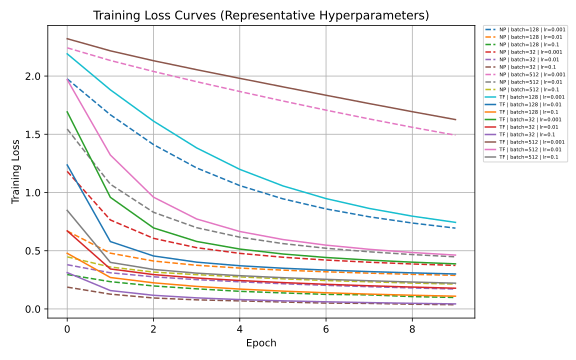
\includegraphics[width=0.85\textwidth]{loss_curves.pdf}
    \caption{Averaged loss curves across epochs for all hyperparameter settings.}
    \label{fig:losscurves}
\end{figure}

\FloatBarrier
\subsection{Summary of Findings}

Across all experiments, the NumPy and TensorFlow implementations exhibited broadly similar accuracy behaviour, with both models showing higher accuracy at larger learning rates and lower accuracy at larger batch sizes. Accuracy trends aligned closely across frameworks, and for many hyperparameter pairs the resulting values were nearly identical.\\

The key differences emerged in training dynamics and runtime. NumPy training times were tightly clustered and largely insensitive to hyperparameters, reflecting Python-level overhead rather than computational throughput. TensorFlow, by contrast, showed clear and systematic speed improvements with larger batch sizes, forming a structured speed–accuracy frontier.\\

Heatmaps and loss curves further highlighted these contrasts. Both models produced smooth and interpretable accuracy heatmaps, but TensorFlow demonstrated much more regular and stable runtime patterns. Loss curves for the two implementations were similar overall, with TensorFlow converging slightly more smoothly and quickly.\\

Overall, the findings show that although both implementations achieve comparable accuracy across the hyperparameter grid, TensorFlow provides more stable optimisation behaviour and substantially more efficient execution, particularly at larger batch sizes, leading to superior scalability.\\


\section{Discussion}
\subsection{Generalisation Patterns}

Across the entire hyperparameter grid, both implementations displayed qualitatively similar trends in generalisation performance. Smaller batch sizes produced higher test accuracies, while large batches tended to underperform unless paired with sufficiently large learning rates. These patterns are consistent with established stochastic gradient descent (SGD) theory, in which small batches introduce gradient noise that acts as an implicit regulariser, promoting convergence to flatter minima associated with better generalisation.\\

Learning rate proved to be the most influential factor in determining final accuracy. Very small learning rates (e.g., 0.001) consistently underfit, failing to make adequate progress even across multiple epochs. Moderately large learning rates (0.03–0.1) yielded the strongest results in both frameworks, enabling the models to escape sharp minima and traverse the loss landscape more effectively. This behaviour suggests that the architecture and dataset fall within the regime where aggressive learning rates are beneficial—a typical property of shallow networks trained on MNIST.\\

\subsection{Computational Efficiency}

The training-time results reveal a fundamental distinction between Python-level numerical computation and framework-optimised tensor execution. In the NumPy implementation, training time remained nearly constant across all batch sizes. The reduction in the number of parameter-update steps at large batch sizes was effectively cancelled out by the increased cost of each iteration. The runtime was dominated by Python overhead—loop execution, memory allocation, and repeated calls into NumPy—which left little room for performance gains from vectorisation alone.\\

TensorFlow, by contrast, exploited hardware acceleration even in a CPU-only environment. Larger batch sizes significantly reduced the number of kernel launches per epoch, allowing the framework to amortise overhead and achieve higher throughput. The underlying C++ and BLAS libraries executed the bulk of the computation, enabling aggressive optimisation strategies such as vectorised operations, cache-aware memory management, and parallel execution of matrix multiplications. As a result, training times decreased sharply as batch size increased, a behaviour entirely absent in the NumPy implementation.\\

These findings underscore the importance of execution strategy in deep learning workloads: the same mathematical operations can produce radically different runtime characteristics depending on how they are scheduled, parallelised, and dispatched.\\

\subsection{Framework-Level Differences}

Beyond raw performance, the two implementations differ structurally in ways that influence optimisation behaviour.
TensorFlow benefits from:
\begin{itemize}
\item	automatic differentiation, ensuring consistent and correctly scaled gradients;
\item kernel fusion, reducing numerical error and improving memory locality in comparison to the NumPy implementation;
\item parallelised tensor execution, leveraging multi-core CPU instructions;
\item static optimisation, such as graph-level analysis in certain execution modes;
\item built-in numerical stabilisation, especially for softmax and cross-entropy.
\end{itemize}

NumPy, while offering transparency and educational clarity, lacks these features. Its gradient computations are manually coded, making them susceptible to subtle implementation errors. Its execution model is inherently sequential, bound to Python’s interpretation overhead. And its numerical routines, although reliable, are not designed to support deep learning workloads that involve repeatedly composing many nonlinear operations over large datasets.\\

These differences explain the smoother convergence, lower variance, and higher efficiency observed in the TensorFlow runs. They also illustrate why modern deep learning research and industry practice overwhelmingly rely on framework-level tooling rather than bespoke NumPy scripts.\\

\subsection{Limitations}

Several limitations constrain the scope of the present study. First, MNIST is a relatively simple dataset. While suitable for controlled comparisons, it does not stress test either framework, nor does it reveal performance characteristics relevant to high-dimensional or highly structured data. More complex datasets—such as CIFAR-10, Fashion-MNIST, or EMNIST—would likely amplify the observed differences.\\

Second, the NumPy implementation uses plain stochastic gradient descent without momentum or adaptive methods. This choice isolates the effects of basic optimisation mechanics but may exaggerate the instability relative to TensorFlow, where optimisers such as Adam or RMSProp are commonly used.\\

Third, all experiments were performed on CPU. TensorFlow’s performance advantage would be substantially greater on GPU-enabled hardware, where kernel-level parallelism plays a far larger role.\\

Finally, although care was taken to script and automate all runs, a completely deterministic comparison is difficult to achieve across different frameworks due to inherent differences in backend scheduling and floating-point execution.\\

Nevertheless, the findings provide a clear and meaningful comparison of the two implementation strategies, demonstrating that even simple architectures can behave very differently depending on the computational substrate on which they are realised.\\


\section{Conclusion}
\subsection{Summary of Findings}

Across all experiments, the NumPy and TensorFlow implementations produced broadly similar accuracy trends: performance increased with learning rate and decreased with batch size, and for many hyperparameter settings the two models achieved nearly identical accuracy. This consistency was reflected in the batch-size and learning-rate comparison plots as well as the accuracy heatmaps, where both frameworks exhibited smooth, interpretable patterns.\\

The main differences arose in training stability and runtime. NumPy training times were tightly clustered and almost entirely unaffected by hyperparameters, indicating that Python overhead dominated its execution. TensorFlow, in contrast, displayed a clear speedup at larger batch sizes and formed a structured speed–accuracy frontier, reflecting efficient use of optimised tensor operations. Heatmaps and loss curves reinforced this distinction: while both implementations converged similarly, TensorFlow was smoother, more stable, and consistently faster at scale. Overall, the results show that although accuracy is comparable between the two implementations, TensorFlow delivers far superior computational efficiency and more reliable optimisation behaviour.\\

\subsection{Implications}

The results highlight several broader implications regarding the practice of machine learning and the engineering of computational tools. First, they underscore the importance of using optimised deep-learning frameworks for any nontrivial workload. Frameworks such as TensorFlow provide not only convenience but also substantial gains in speed, stability, and numerical correctness. These advantages stem from engineered features—automatic differentiation, kernel fusion, parallel execution, and precision management—that are difficult to reproduce in ad hoc implementations.\\

Second, the findings reinforce the educational value of manual implementations. Building an MLP from scratch exposes the full gradient flow, the structure of the computational graph, and the sources of numerical error. This transparency cultivates intuition about optimisation, convergence, and the behaviour of neural networks under different hyperparameters—insights that are often lost when using high-level frameworks exclusively.\\

Third, the experiment holds relevance for real-world data science and quantitative workflows, where reliability and efficiency are essential. In environments such as quantitative finance, algorithmic trading, and large-scale data analytics, predictable runtime behaviour and stable optimisation are vital. The clear superiority of TensorFlow in both aspects suggests that manually coded models are inappropriate for production settings, regardless of the simplicity of the underlying architecture.
More broadly, the results illustrate that even modest neural networks are sensitive to the computational substrate on which they are implemented. Framework-level engineering decisions—rather than architectural design alone—play a decisive role in shaping training dynamics.\\

\subsection{Recommendations}

Based on the findings, the following recommendations can be made for practitioners and students. NumPy-based implementations are most appropriate in educational contexts or when debugging specific components of a learning algorithm. They provide unmatched transparency and allow precise control over every mathematical operation. However, they should not be used for performance-critical workloads or for experiments requiring high numerical stability.\\

TensorFlow (or comparable frameworks) should be preferred for practical training pipelines, exploratory experiments, and any setting where speed, reliability, and reproducibility are priorities. Frameworks provide optimised kernels, automatic differentiation, and ready access to hardware acceleration. These advantages translate directly into improved convergence and generalisation performance, as demonstrated in this study.\\

\subsection{Future Work}

Several natural extensions arise from this study, each offering the potential to deepen our understanding of how implementation choices shape optimisation behaviour. A first direction concerns expanding the scope of architectures. Applying the same comparative analysis to convolutional neural networks would reveal whether the differences observed here persist in models that more closely resemble those used in practical image-recognition systems. Likewise, incorporating more advanced optimisation algorithms—such as momentum-based SGD or Adam—would help determine whether the instability of the NumPy implementation is primarily a consequence of the optimiser or the computational substrate itself.\\

A second avenue involves exploring alternative execution environments. Running the experiments on GPU-enabled hardware would quantify how dramatically the performance gap widens when TensorFlow can exploit large-scale parallelism. Similarly, repeating the analysis on more challenging datasets such as Fashion-MNIST, CIFAR-10, or EMNIST would reveal whether the observed patterns generalise to higher-dimensional or more complex data distributions. Introducing regularisation mechanisms such as dropout, weight decay, or batch normalisation would further enrich the comparison by examining how numerical stability interacts with explicit regularisation strategies.\\

Finally, the growing interest in JAX invites a natural extension of this work. JAX combines NumPy-like syntax with just-in-time compilation and automatic differentiation, potentially offering a brid ge between the educational clarity of manual implementations and the computational efficiency of industrial-grade frameworks. Comparing NumPy, TensorFlow, and JAX on identical architectures would help clarify the trade-off between transparency and performance in modern scientific computing. Investigating mixed-precision training across these systems would extend this comparison into the domain of numerical efficiency.\\

Taken together, these directions outline a broad landscape of future inquiry. Each would enrich the empirical foundation established here and contribute to a more complete understanding of how implementation-level decisions influence not only runtime performance, but also the reliability, stability, and ultimately the scientific utility of machine-learning models.


\newpage
\begin{thebibliography}{9}
\addcontentsline{toc}{section}{Bibliography}

\bibitem{tensorflow}
M. Abadi et al.  
\textit{TensorFlow: Large-Scale Machine Learning on Heterogeneous Systems}, 2015.

\bibitem{mnist}
Y. LeCun, C. Cortes.  
\textit{MNIST Handwritten Digit Database}.  
\url{http://yann.lecun.com/exdb/mnist/}

\end{thebibliography}

\end{document}